\documentclass[a4paper, openany]{memoir}

\usepackage[utf8]{inputenc}
\usepackage[T1]{fontenc} 
\usepackage[english]{babel}

\usepackage{fancyhdr}
\usepackage{float}

\usepackage{amsmath}
\usepackage{amsthm}
\usepackage{amssymb}
\usepackage{enumitem}
\usepackage{multicol}
\usepackage[bookmarksopen=true,bookmarksopenlevel=2]{hyperref}
\usepackage{tikz}
\usepackage{listings}
\usepackage{xcolor}
\usepackage{indentfirst}
\usepackage{caption}
\usepackage{subcaption}

\pagestyle{fancy}
\fancyhf{}
\fancyhead[LE]{\leftmark}
\fancyhead[RO]{\rightmark}
\fancyhead[RE, LO]{Algorithmics II}
\fancyfoot[LE, RO]{\thepage}
\fancyfoot[RE, LO]{Pete Gautam}

\usetikzlibrary{positioning, automata, arrows}

\definecolor{codegreen}{rgb}{0,0.6,0}
\definecolor{codegray}{rgb}{0.5,0.5,0.5}
\definecolor{codepurple}{rgb}{0.58,0,0.82}
\definecolor{backcolour}{rgb}{0.95,0.95,0.92}

\lstdefinestyle{thestyle}{
    backgroundcolor=\color{backcolour},
    basicstyle=\ttfamily\footnotesize,
    keywordstyle=\color{red!80}\bfseries,
    ndkeywordstyle=\color{blue!80}\bfseries,
    identifierstyle=\color{black},
    commentstyle=\color{codegreen},
    stringstyle=\color{codepurple},
    breakatwhitespace=false,
    breaklines=true,
    captionpos=b,
    keepspaces=true,
    numberstyle=\tiny\color{codegray},
    numbers=left,
    numbersep=2pt,
    showspaces=false,
    showstringspaces=false,
    showtabs=false,          
    tabsize=2
}

\lstdefinelanguage{pseudocode}{ 
    keywords={new, return, this, null, if, in, while, else, for, get, set, class, and, or, not, max},
    ndkeywords={int, char, bool, void, double, true, false, Line, LineSegment, Point, Rectangle, List, Map, Edge, Graph, Queue, Vertex},
    sensitive=true,
    comment=[l]{//},
    morecomment=[s]{/*}{*/},
    morestring=[b]',
    morestring=[b]"
}

\lstset{style=thestyle}

\usetikzlibrary{shapes, positioning}

\chapterstyle{thatcher}

\setcounter{chapter}{2}

\begin{document}
    \chapter{Graph and Matching Algorithms}
    \section{Matching in bipartile graphs}
    In this section, we will study a way to produce a matching in bipartile graphs of maximum cardinality, and consider the concept of an augmenting path and why it is important to extend the length of the matching.

    A \emph{bipartile graph} $G$ is a graph $G = (V, E)$, where $V$ can be partitioned to two non-empty subsets $U$ and $W$ such that every edge in $E$ goes from $U$ to $W$. A \emph{matching} in $G$ is a subset $M$ of $E$ such that no two edges have in common. For instance, consider the following figure, showing a matching and not a matching:
    \begin{figure}[H]
        \centering
        \begin{subfigure}{0.45\textwidth}
            \centering
            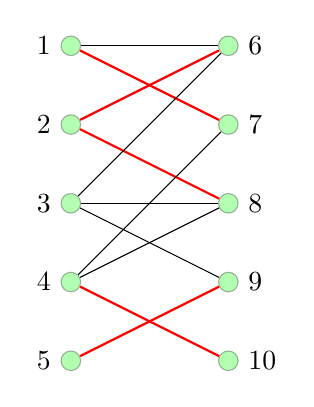
\begin{tikzpicture}
                \node[circle, draw=black, inner sep=2.5pt, fill=green, opacity=0.3, label={180:1}] (1) at (0, 0) {};
                \node[circle, draw=black, inner sep=2.5pt, fill=green, opacity=0.3, label={180:2}] (2) at (0, -1) {};
                \node[circle, draw=black, inner sep=2.5pt, fill=green, opacity=0.3, label={180:3}] (3) at (0, -2) {};
                \node[circle, draw=black, inner sep=2.5pt, fill=green, opacity=0.3, label={180:4}] (4) at (0, -3) {};
                \node[circle, draw=black, inner sep=2.5pt, fill=green, opacity=0.3, label={180:5}] (5) at (0, -4) {};
                \node[circle, draw=black, inner sep=2.5pt, fill=green, opacity=0.3, label={0:6}] (6) at (2, 0) {};
                \node[circle, draw=black, inner sep=2.5pt, fill=green, opacity=0.3, label={0:7}] (7) at (2, -1) {};
                \node[circle, draw=black, inner sep=2.5pt, fill=green, opacity=0.3, label={0:8}] (8) at (2, -2) {};
                \node[circle, draw=black, inner sep=2.5pt, fill=green, opacity=0.3, label={0:9}] (9) at (2, -3) {};
                \node[circle, draw=black, inner sep=2.5pt, fill=green, opacity=0.3, label={0:10}] (10) at (2, -4) {};
            
                \draw (1) -- (6);
                \draw[red, thick] (1) -- (7);
                \draw[red, thick] (2) -- (6);
                \draw[red, thick] (2) -- (8);
                \draw (3) -- (6);
                \draw (3) -- (8);
                \draw (3) -- (9);
                \draw (4) -- (7);
                \draw (4) -- (8);
                \draw[red, thick] (4) -- (10);
                \draw[red, thick] (5) -- (9);
            \end{tikzpicture}
            \caption{Not a matching- vertex 2 has 2 matching edges}
        \end{subfigure}
        \hfill
        \begin{subfigure}{0.45\textwidth}
            \centering
            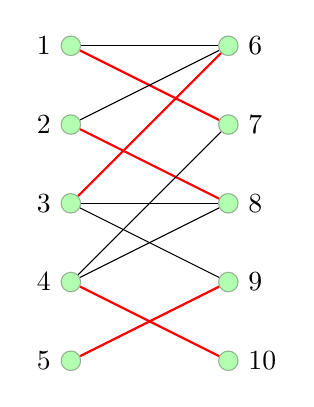
\begin{tikzpicture}
                \node[circle, draw=black, inner sep=2.5pt, fill=green, opacity=0.3, label={180:1}] (1) at (0, 0) {};
                \node[circle, draw=black, inner sep=2.5pt, fill=green, opacity=0.3, label={180:2}] (2) at (0, -1) {};
                \node[circle, draw=black, inner sep=2.5pt, fill=green, opacity=0.3, label={180:3}] (3) at (0, -2) {};
                \node[circle, draw=black, inner sep=2.5pt, fill=green, opacity=0.3, label={180:4}] (4) at (0, -3) {};
                \node[circle, draw=black, inner sep=2.5pt, fill=green, opacity=0.3, label={180:5}] (5) at (0, -4) {};
                \node[circle, draw=black, inner sep=2.5pt, fill=green, opacity=0.3, label={0:6}] (6) at (2, 0) {};
                \node[circle, draw=black, inner sep=2.5pt, fill=green, opacity=0.3, label={0:7}] (7) at (2, -1) {};
                \node[circle, draw=black, inner sep=2.5pt, fill=green, opacity=0.3, label={0:8}] (8) at (2, -2) {};
                \node[circle, draw=black, inner sep=2.5pt, fill=green, opacity=0.3, label={0:9}] (9) at (2, -3) {};
                \node[circle, draw=black, inner sep=2.5pt, fill=green, opacity=0.3, label={0:10}] (10) at (2, -4) {};
            
                \draw (1) -- (6);
                \draw[red, thick] (1) -- (7);
                \draw (2) -- (6);
                \draw[red, thick] (2) -- (8);
                \draw[red, thick] (3) -- (6);
                \draw (3) -- (8);
                \draw (3) -- (9);
                \draw (4) -- (7);
                \draw (4) -- (8);
                \draw[red, thick] (4) -- (10);
                \draw[red, thick] (5) -- (9);
            \end{tikzpicture}
            \caption{A matching}
        \end{subfigure}
    \end{figure}
    \noindent A \emph{maximum cardinality matching} is a matching that has the highest number of edges. A maximum matching is \emph{perfect} if it has cardinality $|V|/2$, i.e. every vertex is part of some edge in the matching. The example above shows a perfect matching. Not every bipartile graph has a perfect matching, such as the graph below:
    \begin{figure}[H]
        \centering
        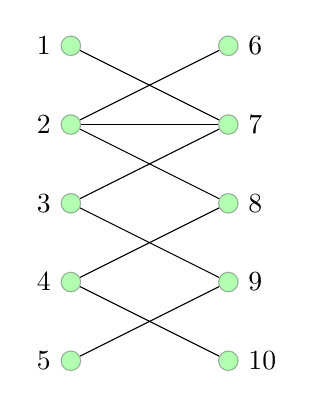
\begin{tikzpicture}
            \node[circle, draw=black, inner sep=2.5pt, fill=green, opacity=0.3, label={180:1}] (1) at (0, 0) {};
            \node[circle, draw=black, inner sep=2.5pt, fill=green, opacity=0.3, label={180:2}] (2) at (0, -1) {};
            \node[circle, draw=black, inner sep=2.5pt, fill=green, opacity=0.3, label={180:3}] (3) at (0, -2) {};
            \node[circle, draw=black, inner sep=2.5pt, fill=green, opacity=0.3, label={180:4}] (4) at (0, -3) {};
            \node[circle, draw=black, inner sep=2.5pt, fill=green, opacity=0.3, label={180:5}] (5) at (0, -4) {};
            \node[circle, draw=black, inner sep=2.5pt, fill=green, opacity=0.3, label={0:6}] (6) at (2, 0) {};
            \node[circle, draw=black, inner sep=2.5pt, fill=green, opacity=0.3, label={0:7}] (7) at (2, -1) {};
            \node[circle, draw=black, inner sep=2.5pt, fill=green, opacity=0.3, label={0:8}] (8) at (2, -2) {};
            \node[circle, draw=black, inner sep=2.5pt, fill=green, opacity=0.3, label={0:9}] (9) at (2, -3) {};
            \node[circle, draw=black, inner sep=2.5pt, fill=green, opacity=0.3, label={0:10}] (10) at (2, -4) {};
        
            \draw (1) -- (7);
            \draw (2) -- (6);
            \draw (2) -- (7);
            \draw (2) -- (8);
            \draw (3) -- (7);
            \draw (3) -- (9);
            \draw (4) -- (8);
            \draw (4) -- (10);
            \draw (5) -- (9);
        \end{tikzpicture}
    \end{figure}
    \noindent We will prove this by a contradiction. So, assume that this graph has a perfect matching. In that case, every vertex with just 1 edge will be part of the matching subset. This means that the red edges given below are part of the matching subset:
    \begin{figure}[H]
        \centering
        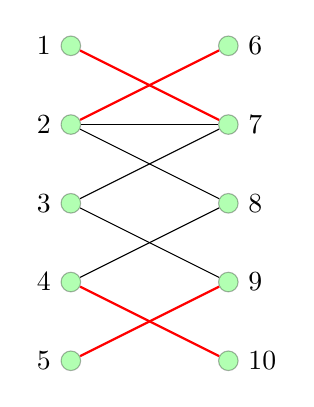
\begin{tikzpicture}
            \node[circle, draw=black, inner sep=2.5pt, fill=green, opacity=0.3, label={180:1}] (1) at (0, 0) {};
            \node[circle, draw=black, inner sep=2.5pt, fill=green, opacity=0.3, label={180:2}] (2) at (0, -1) {};
            \node[circle, draw=black, inner sep=2.5pt, fill=green, opacity=0.3, label={180:3}] (3) at (0, -2) {};
            \node[circle, draw=black, inner sep=2.5pt, fill=green, opacity=0.3, label={180:4}] (4) at (0, -3) {};
            \node[circle, draw=black, inner sep=2.5pt, fill=green, opacity=0.3, label={180:5}] (5) at (0, -4) {};
            \node[circle, draw=black, inner sep=2.5pt, fill=green, opacity=0.3, label={0:6}] (6) at (2, 0) {};
            \node[circle, draw=black, inner sep=2.5pt, fill=green, opacity=0.3, label={0:7}] (7) at (2, -1) {};
            \node[circle, draw=black, inner sep=2.5pt, fill=green, opacity=0.3, label={0:8}] (8) at (2, -2) {};
            \node[circle, draw=black, inner sep=2.5pt, fill=green, opacity=0.3, label={0:9}] (9) at (2, -3) {};
            \node[circle, draw=black, inner sep=2.5pt, fill=green, opacity=0.3, label={0:10}] (10) at (2, -4) {};
        
            \draw[red, thick] (1) -- (7);
            \draw[red, thick] (2) -- (6);
            \draw (2) -- (7);
            \draw (2) -- (8);
            \draw (3) -- (7);
            \draw (3) -- (9);
            \draw (4) -- (8);
            \draw[red, thick] (4) -- (10);
            \draw[red, thick] (5) -- (9);
        \end{tikzpicture}
    \end{figure}
    \noindent Now, since there is a perfect matching, we must be able to add precisely one further edge that will incorporate both the vertices 3 and 8. However, there is no edge between 3 and 8, and adding any other edge would only incorporate one of the vertices (and break the match property). So, this graph does not have a perfect matching. In fact, what we have above is the maximum cardinality matching for the graph.
    
    We will now construct an algorithm to compute the edges that form a maximum cardinality matching. If we did this using brute force, we would need to go through all the permutation of the edges and check whether it is a matching, and if so, whether it is also the maximum (up to that point during the algorithm). This will take $O(m!)$ time, where $m$ is the number of edges in the graph, and is essentially intractable. 

    We shall now look for a better algorithm, which has complexity $O(m^3)$. This uses the concept of finding an \emph{augmenting path} in the current matching to increase, if possible, the size of the matching by 1. The advantage we have in this case is that if we cannot find an augmenting path, then we have found the maximum cardinality matching. At the start, we have an empty matching, from which we increment the size of the matching by 1 until this is not possible, by finding an augmenting path.

    Before defining an augmenting path, we illustrate how this works. So, assume that we are at the following matching:
    \begin{figure}[H]
        \centering
        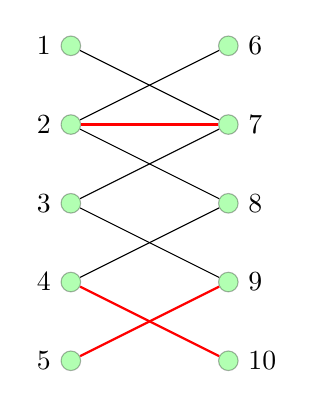
\begin{tikzpicture}
            \node[circle, draw=black, inner sep=2.5pt, fill=green, opacity=0.3, label={180:1}] (1) at (0, 0) {};
            \node[circle, draw=black, inner sep=2.5pt, fill=green, opacity=0.3, label={180:2}] (2) at (0, -1) {};
            \node[circle, draw=black, inner sep=2.5pt, fill=green, opacity=0.3, label={180:3}] (3) at (0, -2) {};
            \node[circle, draw=black, inner sep=2.5pt, fill=green, opacity=0.3, label={180:4}] (4) at (0, -3) {};
            \node[circle, draw=black, inner sep=2.5pt, fill=green, opacity=0.3, label={180:5}] (5) at (0, -4) {};
            \node[circle, draw=black, inner sep=2.5pt, fill=green, opacity=0.3, label={0:6}] (6) at (2, 0) {};
            \node[circle, draw=black, inner sep=2.5pt, fill=green, opacity=0.3, label={0:7}] (7) at (2, -1) {};
            \node[circle, draw=black, inner sep=2.5pt, fill=green, opacity=0.3, label={0:8}] (8) at (2, -2) {};
            \node[circle, draw=black, inner sep=2.5pt, fill=green, opacity=0.3, label={0:9}] (9) at (2, -3) {};
            \node[circle, draw=black, inner sep=2.5pt, fill=green, opacity=0.3, label={0:10}] (10) at (2, -4) {};
        
            \draw (1) -- (7);
            \draw (2) -- (6);
            \draw[red, thick] (2) -- (7);
            \draw (2) -- (8);
            \draw (3) -- (7);
            \draw (3) -- (9);
            \draw (4) -- (8);
            \draw[red, thick] (4) -- (10);
            \draw[red, thick] (5) -- (9);
        \end{tikzpicture}
    \end{figure}
    \noindent We can find an augmenting path here, which is shown below.
    \begin{figure}[H]
        \centering
        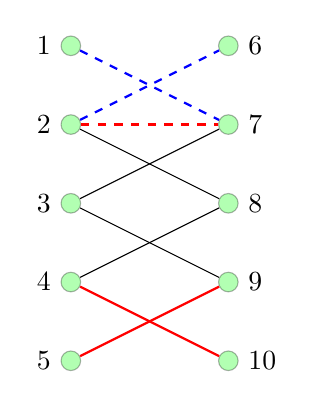
\begin{tikzpicture}
            \node[circle, draw=black, inner sep=2.5pt, fill=green, opacity=0.3, label={180:1}] (1) at (0, 0) {};
            \node[circle, draw=black, inner sep=2.5pt, fill=green, opacity=0.3, label={180:2}] (2) at (0, -1) {};
            \node[circle, draw=black, inner sep=2.5pt, fill=green, opacity=0.3, label={180:3}] (3) at (0, -2) {};
            \node[circle, draw=black, inner sep=2.5pt, fill=green, opacity=0.3, label={180:4}] (4) at (0, -3) {};
            \node[circle, draw=black, inner sep=2.5pt, fill=green, opacity=0.3, label={180:5}] (5) at (0, -4) {};
            \node[circle, draw=black, inner sep=2.5pt, fill=green, opacity=0.3, label={0:6}] (6) at (2, 0) {};
            \node[circle, draw=black, inner sep=2.5pt, fill=green, opacity=0.3, label={0:7}] (7) at (2, -1) {};
            \node[circle, draw=black, inner sep=2.5pt, fill=green, opacity=0.3, label={0:8}] (8) at (2, -2) {};
            \node[circle, draw=black, inner sep=2.5pt, fill=green, opacity=0.3, label={0:9}] (9) at (2, -3) {};
            \node[circle, draw=black, inner sep=2.5pt, fill=green, opacity=0.3, label={0:10}] (10) at (2, -4) {};
        
            \draw[blue, thick, dashed] (1) -- (7);
            \draw[blue, thick, dashed] (2) -- (6);
            \draw[red, dashed, thick] (2) -- (7);
            \draw (2) -- (8);
            \draw (3) -- (7);
            \draw (3) -- (9);
            \draw (4) -- (8);
            \draw[red, thick] (4) -- (10);
            \draw[red, thick] (5) -- (9);
        \end{tikzpicture}
    \end{figure}
    \noindent The augmenting path is the dashed path from the vertex 1 to 6 (or vice versa). An augmenting path alternates between edges in the match and not in the match, and helps us extend the cardinality of the matching. In this case, we remove the edge 2-7 from the matching (the dashed red edge), and replace it with 1-7 and 2-6 (the dashed blue edges). This gives us the following matching:
    \begin{figure}[H]
        \centering
        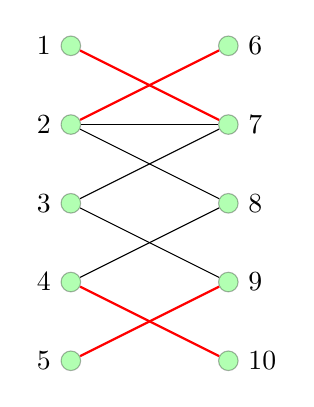
\begin{tikzpicture}
            \node[circle, draw=black, inner sep=2.5pt, fill=green, opacity=0.3, label={180:1}] (1) at (0, 0) {};
            \node[circle, draw=black, inner sep=2.5pt, fill=green, opacity=0.3, label={180:2}] (2) at (0, -1) {};
            \node[circle, draw=black, inner sep=2.5pt, fill=green, opacity=0.3, label={180:3}] (3) at (0, -2) {};
            \node[circle, draw=black, inner sep=2.5pt, fill=green, opacity=0.3, label={180:4}] (4) at (0, -3) {};
            \node[circle, draw=black, inner sep=2.5pt, fill=green, opacity=0.3, label={180:5}] (5) at (0, -4) {};
            \node[circle, draw=black, inner sep=2.5pt, fill=green, opacity=0.3, label={0:6}] (6) at (2, 0) {};
            \node[circle, draw=black, inner sep=2.5pt, fill=green, opacity=0.3, label={0:7}] (7) at (2, -1) {};
            \node[circle, draw=black, inner sep=2.5pt, fill=green, opacity=0.3, label={0:8}] (8) at (2, -2) {};
            \node[circle, draw=black, inner sep=2.5pt, fill=green, opacity=0.3, label={0:9}] (9) at (2, -3) {};
            \node[circle, draw=black, inner sep=2.5pt, fill=green, opacity=0.3, label={0:10}] (10) at (2, -4) {};
        
            \draw[red, thick] (1) -- (7);
            \draw[red, thick] (2) -- (6);
            \draw (2) -- (7);
            \draw (2) -- (8);
            \draw (3) -- (7);
            \draw (3) -- (9);
            \draw (4) -- (8);
            \draw[red, thick] (4) -- (10);
            \draw[red, thick] (5) -- (9);
        \end{tikzpicture}
    \end{figure}
    \noindent As we were able to find an augmenting path, we have been able to extend the matching subset by 1.

    We now build to the definition of augmenting path. In a matching $M$, we say that a vertex $v$ is \emph{matching} if it is part of some edge in the matching subset. If the edge goes from $v$ to $u$, then we say that $u$ and $v$ are \emph{mates}. If the vertex $v$ is not matched, then it is \emph{exposed}. An \emph{alternating path} alternates between edges in $M$ and edges not in $M$. An \emph{augmenting path} is an alternating path that starts and ends at exposed vertices.

    An augmenting path allows us to increase the length of the matching subset- an augmenting path has odd length (if it had even length, then it must end at an exposed vertex), so there is one more non-matching edge in the augmenting path than a matching edge. So, when we replace the matching edges with the non-matching edges, we still have a match (we are swapping the mates for the exposed vertices, and the unexposed vertices originally had no match). Moreover, if there is no augmenting path from any of the unexposed vertices, then we are at a maximum cardinality match.

    We will now consider the algorithm in general.
\begin{lstlisting}[language=pseudocode]
List<Edge> maximumMatching(Graph graph) {
    List<Edge> matching = [];
    Vertex augmentedPath = getAugmentedPath(graph.leftVertices);
    while (augmentedPath != null) {
        matching = augment(augmentedPath);
        augmentedPath = graph.getAugmentedPath();
    }
    return matching;
}
\end{lstlisting}
    The function \texttt{getAugmentedPath} tries to find an augmented path in the bipartile graph given its `left' vertices, and returns the final vertex in the path. The function \texttt{augment} takes an augmented path and selects the right edges to add to the matching.

    Next, we look at the method \texttt{getAugmentedPath} in detail. It is based on breadth-first search, starting from an unexposed vertex until we get to an unexposed vertex `on the same side'. As we saw in the algorithm above, we will only have a look at the left vertices. The following is the algorithm:
\begin{lstlisting}[language=pseudocode]
Vertex getAugmentedPath(List<Vertex> leftVertices) {
    Vertex startVertex = leftVertices.first((v) => v.isUnexposed);
    // no startVertex => every left vertex is exposed 
    if (startVertex == null) {
        return null;
    }

    // Do a DFS to find an unexposed vertex
    Queue<Vertex> queue = Queue(startVertex);
    while (queue.isNotEmpty) {
        Vertex vertex = queue.remove();
        List<Edge> edges = vertex.edges;

        for (int i=0; i<edges.length; i++) {
            Vertex range = edges[i].range;
            if (range.isVisited) {
                range.predecessorEdge = edges[i];
                if (range.isUnexposed) {
                    return range;
                } else {
                    queue.add(range.mate);
                }
            }
        }
    }

    // not possible to find a path between two unexposed vertices
    return null;
}
\end{lstlisting}
    We can then \texttt{augment} to find the matching path as follows:
\begin{lstlisting}[language=pseudocode]
List<Edge> augment(Vertex endVertex) {
    List<Edge> edges = [];
    Vertex vertex = endVertex;
    Edge edge = endVertex.predecessorEdge;

    while (edge != null) {
        Vertex temp = edge.range.mate;
        edge.range.mate = vertex;
        vertex.mate = edge.range;
        edges.add(edge);

        vertex = temp;
        edge = vertex.predecessorEdge;
    }

    return edges;
}
\end{lstlisting}
    Note that the variable \texttt{vertex} at line 12 cannot be null since it is on the left (and the path goes from a left vertex to another left vertex).

    We will now illustrate how the algorithm works with an example. So, assume that we have the following graph.
    \begin{figure}[H]
        \centering
        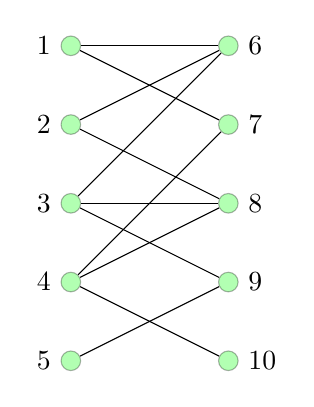
\begin{tikzpicture}
            \node[circle, draw=black, inner sep=2.5pt, fill=green, opacity=0.3, label={180:1}] (1) at (0, 0) {};
            \node[circle, draw=black, inner sep=2.5pt, fill=green, opacity=0.3, label={180:2}] (2) at (0, -1) {};
            \node[circle, draw=black, inner sep=2.5pt, fill=green, opacity=0.3, label={180:3}] (3) at (0, -2) {};
            \node[circle, draw=black, inner sep=2.5pt, fill=green, opacity=0.3, label={180:4}] (4) at (0, -3) {};
            \node[circle, draw=black, inner sep=2.5pt, fill=green, opacity=0.3, label={180:5}] (5) at (0, -4) {};
            \node[circle, draw=black, inner sep=2.5pt, fill=green, opacity=0.3, label={0:6}] (6) at (2, 0) {};
            \node[circle, draw=black, inner sep=2.5pt, fill=green, opacity=0.3, label={0:7}] (7) at (2, -1) {};
            \node[circle, draw=black, inner sep=2.5pt, fill=green, opacity=0.3, label={0:8}] (8) at (2, -2) {};
            \node[circle, draw=black, inner sep=2.5pt, fill=green, opacity=0.3, label={0:9}] (9) at (2, -3) {};
            \node[circle, draw=black, inner sep=2.5pt, fill=green, opacity=0.3, label={0:10}] (10) at (2, -4) {};
        
            \draw (1) -- (6);
            \draw (1) -- (7);
            \draw (2) -- (6);
            \draw (2) -- (8);
            \draw (3) -- (6);
            \draw (3) -- (8);
            \draw (3) -- (9);
            \draw (4) -- (7);
            \draw (4) -- (8);
            \draw (4) -- (10);
            \draw (5) -- (9);
        \end{tikzpicture}
    \end{figure}
    \noindent At the start, we have the empty matching. We will find an augmenting path in the graph.
    \begin{figure}[H]
        \centering
        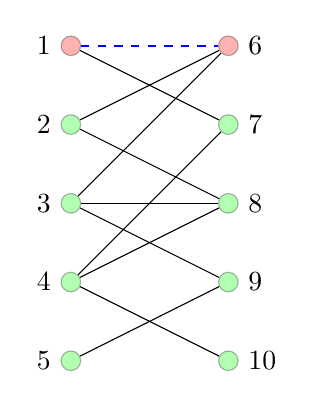
\begin{tikzpicture}
            \node[circle, draw=black, inner sep=2.5pt, fill=red, opacity=0.3, label={180:1}] (1) at (0, 0) {};
            \node[circle, draw=black, inner sep=2.5pt, fill=green, opacity=0.3, label={180:2}] (2) at (0, -1) {};
            \node[circle, draw=black, inner sep=2.5pt, fill=green, opacity=0.3, label={180:3}] (3) at (0, -2) {};
            \node[circle, draw=black, inner sep=2.5pt, fill=green, opacity=0.3, label={180:4}] (4) at (0, -3) {};
            \node[circle, draw=black, inner sep=2.5pt, fill=green, opacity=0.3, label={180:5}] (5) at (0, -4) {};
            \node[circle, draw=black, inner sep=2.5pt, fill=red, opacity=0.3, label={0:6}] (6) at (2, 0) {};
            \node[circle, draw=black, inner sep=2.5pt, fill=green, opacity=0.3, label={0:7}] (7) at (2, -1) {};
            \node[circle, draw=black, inner sep=2.5pt, fill=green, opacity=0.3, label={0:8}] (8) at (2, -2) {};
            \node[circle, draw=black, inner sep=2.5pt, fill=green, opacity=0.3, label={0:9}] (9) at (2, -3) {};
            \node[circle, draw=black, inner sep=2.5pt, fill=green, opacity=0.3, label={0:10}] (10) at (2, -4) {};
        
            \draw[blue, dashed, thick] (1) -- (6);
            \draw (1) -- (7);
            \draw (2) -- (6);
            \draw (2) -- (8);
            \draw (3) -- (6);
            \draw (3) -- (8);
            \draw (3) -- (9);
            \draw (4) -- (7);
            \draw (4) -- (8);
            \draw (4) -- (10);
            \draw (5) -- (9);
        \end{tikzpicture}
    \end{figure}
    \noindent We denote by red a visited vertex during this iteration. The first unexposed vertex we find is vertex 1, which has an edge to vertex 6. So, we add this edge to the matching. This gives us the following matching.
    \begin{figure}[H]
        \centering
        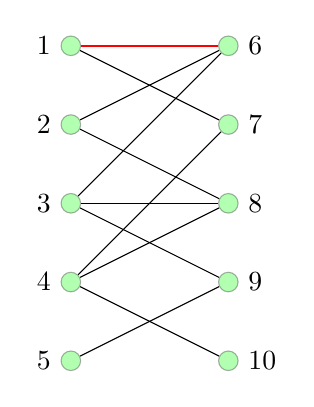
\begin{tikzpicture}
            \node[circle, draw=black, inner sep=2.5pt, fill=green, opacity=0.3, label={180:1}] (1) at (0, 0) {};
            \node[circle, draw=black, inner sep=2.5pt, fill=green, opacity=0.3, label={180:2}] (2) at (0, -1) {};
            \node[circle, draw=black, inner sep=2.5pt, fill=green, opacity=0.3, label={180:3}] (3) at (0, -2) {};
            \node[circle, draw=black, inner sep=2.5pt, fill=green, opacity=0.3, label={180:4}] (4) at (0, -3) {};
            \node[circle, draw=black, inner sep=2.5pt, fill=green, opacity=0.3, label={180:5}] (5) at (0, -4) {};
            \node[circle, draw=black, inner sep=2.5pt, fill=green, opacity=0.3, label={0:6}] (6) at (2, 0) {};
            \node[circle, draw=black, inner sep=2.5pt, fill=green, opacity=0.3, label={0:7}] (7) at (2, -1) {};
            \node[circle, draw=black, inner sep=2.5pt, fill=green, opacity=0.3, label={0:8}] (8) at (2, -2) {};
            \node[circle, draw=black, inner sep=2.5pt, fill=green, opacity=0.3, label={0:9}] (9) at (2, -3) {};
            \node[circle, draw=black, inner sep=2.5pt, fill=green, opacity=0.3, label={0:10}] (10) at (2, -4) {};
        
            \draw[red, thick] (1) -- (6);
            \draw (1) -- (7);
            \draw (2) -- (6);
            \draw (2) -- (8);
            \draw (3) -- (6);
            \draw (3) -- (8);
            \draw (3) -- (9);
            \draw (4) -- (7);
            \draw (4) -- (8);
            \draw (4) -- (10);
            \draw (5) -- (9);
        \end{tikzpicture}
    \end{figure}
    \noindent We will now search for another augmenting path.
    \begin{figure}[H]
        \centering
        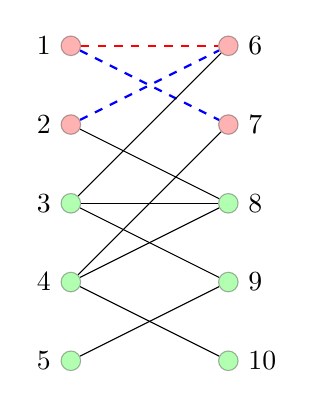
\begin{tikzpicture}
            \node[circle, draw=black, inner sep=2.5pt, fill=red, opacity=0.3, label={180:1}] (1) at (0, 0) {};
            \node[circle, draw=black, inner sep=2.5pt, fill=red, opacity=0.3, label={180:2}] (2) at (0, -1) {};
            \node[circle, draw=black, inner sep=2.5pt, fill=green, opacity=0.3, label={180:3}] (3) at (0, -2) {};
            \node[circle, draw=black, inner sep=2.5pt, fill=green, opacity=0.3, label={180:4}] (4) at (0, -3) {};
            \node[circle, draw=black, inner sep=2.5pt, fill=green, opacity=0.3, label={180:5}] (5) at (0, -4) {};
            \node[circle, draw=black, inner sep=2.5pt, fill=red, opacity=0.3, label={0:6}] (6) at (2, 0) {};
            \node[circle, draw=black, inner sep=2.5pt, fill=red, opacity=0.3, label={0:7}] (7) at (2, -1) {};
            \node[circle, draw=black, inner sep=2.5pt, fill=green, opacity=0.3, label={0:8}] (8) at (2, -2) {};
            \node[circle, draw=black, inner sep=2.5pt, fill=green, opacity=0.3, label={0:9}] (9) at (2, -3) {};
            \node[circle, draw=black, inner sep=2.5pt, fill=green, opacity=0.3, label={0:10}] (10) at (2, -4) {};
        
            \draw[red, dashed, thick] (1) -- (6);
            \draw[blue, dashed, thick] (1) -- (7);
            \draw[blue, dashed, thick] (2) -- (6);
            \draw (2) -- (8);
            \draw (3) -- (6);
            \draw (3) -- (8);
            \draw (3) -- (9);
            \draw (4) -- (7);
            \draw (4) -- (8);
            \draw (4) -- (10);
            \draw (5) -- (9);
        \end{tikzpicture}
    \end{figure}
    \noindent In this case, the augmenting path starts at vertex 2. We first find its edge to vertex 6. This is an exposed vertex, so we add its mate vertex 1 to the queue. From vertex 1, we cannot take the edge to vertex 6 since it has already been visited, so we take the edge to vertex 7. This vertex is exposed, so the augmenting path is complete. Using this, we get the following matching:
    \begin{figure}[H]
        \centering
        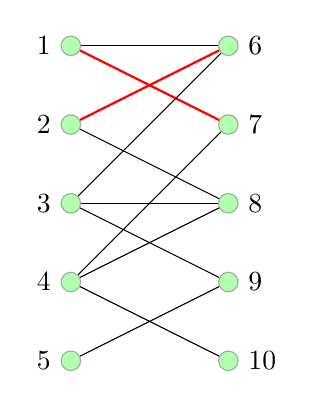
\begin{tikzpicture}
            \node[circle, draw=black, inner sep=2.5pt, fill=green, opacity=0.3, label={180:1}] (1) at (0, 0) {};
            \node[circle, draw=black, inner sep=2.5pt, fill=green, opacity=0.3, label={180:2}] (2) at (0, -1) {};
            \node[circle, draw=black, inner sep=2.5pt, fill=green, opacity=0.3, label={180:3}] (3) at (0, -2) {};
            \node[circle, draw=black, inner sep=2.5pt, fill=green, opacity=0.3, label={180:4}] (4) at (0, -3) {};
            \node[circle, draw=black, inner sep=2.5pt, fill=green, opacity=0.3, label={180:5}] (5) at (0, -4) {};
            \node[circle, draw=black, inner sep=2.5pt, fill=green, opacity=0.3, label={0:6}] (6) at (2, 0) {};
            \node[circle, draw=black, inner sep=2.5pt, fill=green, opacity=0.3, label={0:7}] (7) at (2, -1) {};
            \node[circle, draw=black, inner sep=2.5pt, fill=green, opacity=0.3, label={0:8}] (8) at (2, -2) {};
            \node[circle, draw=black, inner sep=2.5pt, fill=green, opacity=0.3, label={0:9}] (9) at (2, -3) {};
            \node[circle, draw=black, inner sep=2.5pt, fill=green, opacity=0.3, label={0:10}] (10) at (2, -4) {};
        
            \draw (1) -- (6);
            \draw[red, thick] (1) -- (7);
            \draw[red, thick] (2) -- (6);
            \draw (2) -- (8);
            \draw (3) -- (6);
            \draw (3) -- (8);
            \draw (3) -- (9);
            \draw (4) -- (7);
            \draw (4) -- (8);
            \draw (4) -- (10);
            \draw (5) -- (9);
        \end{tikzpicture}
    \end{figure}
    \noindent We can continue using the augmenting algorithm to get to the following matching:
    \begin{figure}[H]
        \centering
        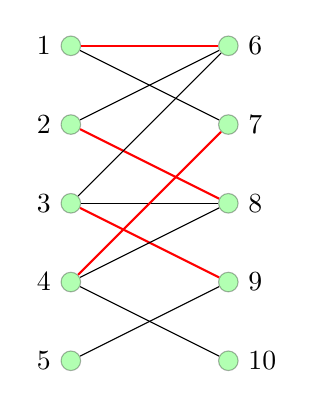
\begin{tikzpicture}
            \node[circle, draw=black, inner sep=2.5pt, fill=green, opacity=0.3, label={180:1}] (1) at (0, 0) {};
            \node[circle, draw=black, inner sep=2.5pt, fill=green, opacity=0.3, label={180:2}] (2) at (0, -1) {};
            \node[circle, draw=black, inner sep=2.5pt, fill=green, opacity=0.3, label={180:3}] (3) at (0, -2) {};
            \node[circle, draw=black, inner sep=2.5pt, fill=green, opacity=0.3, label={180:4}] (4) at (0, -3) {};
            \node[circle, draw=black, inner sep=2.5pt, fill=green, opacity=0.3, label={180:5}] (5) at (0, -4) {};
            \node[circle, draw=black, inner sep=2.5pt, fill=green, opacity=0.3, label={0:6}] (6) at (2, 0) {};
            \node[circle, draw=black, inner sep=2.5pt, fill=green, opacity=0.3, label={0:7}] (7) at (2, -1) {};
            \node[circle, draw=black, inner sep=2.5pt, fill=green, opacity=0.3, label={0:8}] (8) at (2, -2) {};
            \node[circle, draw=black, inner sep=2.5pt, fill=green, opacity=0.3, label={0:9}] (9) at (2, -3) {};
            \node[circle, draw=black, inner sep=2.5pt, fill=green, opacity=0.3, label={0:10}] (10) at (2, -4) {};
        
            \draw[red, thick] (1) -- (6);
            \draw (1) -- (7);
            \draw (2) -- (6);
            \draw[red, thick] (2) -- (8);
            \draw (3) -- (6);
            \draw (3) -- (8);
            \draw[red, thick] (3) -- (9);
            \draw[red, thick] (4) -- (7);
            \draw (4) -- (8);
            \draw (4) -- (10);
            \draw (5) -- (9);
        \end{tikzpicture}
    \end{figure}    
    \noindent Now, we will try finding another augmenting path.
    \begin{figure}[H]
        \centering
        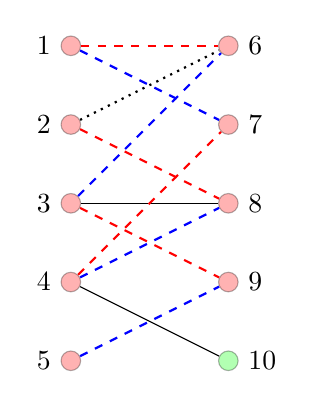
\begin{tikzpicture}
            \node[circle, draw=black, inner sep=2.5pt, fill=red, opacity=0.3, label={180:1}] (1) at (0, 0) {};
            \node[circle, draw=black, inner sep=2.5pt, fill=red, opacity=0.3, label={180:2}] (2) at (0, -1) {};
            \node[circle, draw=black, inner sep=2.5pt, fill=red, opacity=0.3, label={180:3}] (3) at (0, -2) {};
            \node[circle, draw=black, inner sep=2.5pt, fill=red, opacity=0.3, label={180:4}] (4) at (0, -3) {};
            \node[circle, draw=black, inner sep=2.5pt, fill=red, opacity=0.3, label={180:5}] (5) at (0, -4) {};
            \node[circle, draw=black, inner sep=2.5pt, fill=red, opacity=0.3, label={0:6}] (6) at (2, 0) {};
            \node[circle, draw=black, inner sep=2.5pt, fill=red, opacity=0.3, label={0:7}] (7) at (2, -1) {};
            \node[circle, draw=black, inner sep=2.5pt, fill=red, opacity=0.3, label={0:8}] (8) at (2, -2) {};
            \node[circle, draw=black, inner sep=2.5pt, fill=red, opacity=0.3, label={0:9}] (9) at (2, -3) {};
            \node[circle, draw=black, inner sep=2.5pt, fill=green, opacity=0.3, label={0:10}] (10) at (2, -4) {};
        
            \draw[red, dashed, thick] (1) -- (6);
            \draw[blue, dashed, thick] (1) -- (7);
            \draw[dotted, thick] (2) -- (6);
            \draw[red, dashed, thick] (2) -- (8);
            \draw[blue, thick, dashed] (3) -- (6);
            \draw (3) -- (8);
            \draw[red, dashed, thick] (3) -- (9);
            \draw[red, dashed, thick] (4) -- (7);
            \draw[blue, dashed, thick] (4) -- (8);
            \draw (4) -- (10);
            \draw[blue, thick, dashed] (5) -- (9);
        \end{tikzpicture}
    \end{figure}
    \noindent We start with the unexposed vertex 5, and take its edge to vertex 9. This is exposed, so we add its mate to the queue. This process continues as expected, until we add vertex 4 to the queue. We first take the edge it has to vertex 8, at which point we add vertex 3 to the queue. However, every edge that vertex 2 has goes to a visited vertex. So, we have to backtrack- we take the other edge from vertex 4.
    \begin{figure}[H]
        \centering
        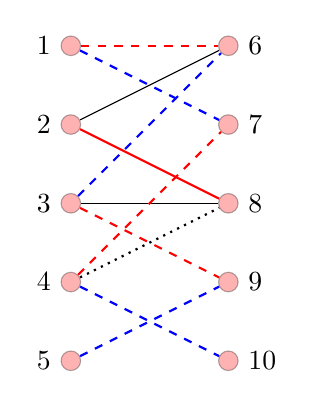
\begin{tikzpicture}
            \node[circle, draw=black, inner sep=2.5pt, fill=red, opacity=0.3, label={180:1}] (1) at (0, 0) {};
            \node[circle, draw=black, inner sep=2.5pt, fill=red, opacity=0.3, label={180:2}] (2) at (0, -1) {};
            \node[circle, draw=black, inner sep=2.5pt, fill=red, opacity=0.3, label={180:3}] (3) at (0, -2) {};
            \node[circle, draw=black, inner sep=2.5pt, fill=red, opacity=0.3, label={180:4}] (4) at (0, -3) {};
            \node[circle, draw=black, inner sep=2.5pt, fill=red, opacity=0.3, label={180:5}] (5) at (0, -4) {};
            \node[circle, draw=black, inner sep=2.5pt, fill=red, opacity=0.3, label={0:6}] (6) at (2, 0) {};
            \node[circle, draw=black, inner sep=2.5pt, fill=red, opacity=0.3, label={0:7}] (7) at (2, -1) {};
            \node[circle, draw=black, inner sep=2.5pt, fill=red, opacity=0.3, label={0:8}] (8) at (2, -2) {};
            \node[circle, draw=black, inner sep=2.5pt, fill=red, opacity=0.3, label={0:9}] (9) at (2, -3) {};
            \node[circle, draw=black, inner sep=2.5pt, fill=red, opacity=0.3, label={0:10}] (10) at (2, -4) {};
        
            \draw[red, dashed, thick] (1) -- (6);
            \draw[blue, dashed, thick] (1) -- (7);
            \draw (2) -- (6);
            \draw[red, thick] (2) -- (8);
            \draw[blue, thick, dashed] (3) -- (6);
            \draw (3) -- (8);
            \draw[red, dashed, thick] (3) -- (9);
            \draw[red, dashed, thick] (4) -- (7);
            \draw[thick, dotted] (4) -- (8);
            \draw[blue, dashed, thick] (4) -- (10);
            \draw[blue, thick, dashed] (5) -- (9);
        \end{tikzpicture}
    \end{figure}
    \noindent In this case, we take the edge from vertex 4 to vertex 10. This is an exposed vertex, so we have found the augmenting path. Moreover, there is no unexposed (left) vertex, so the algorithm terminates with the following matching:
    \begin{figure}[H]
        \centering
        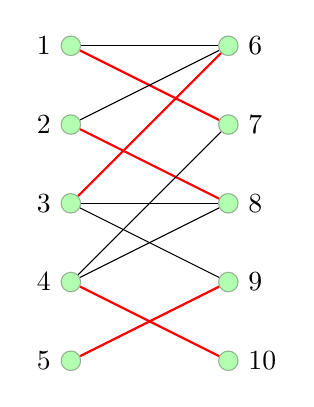
\begin{tikzpicture}
            \node[circle, draw=black, inner sep=2.5pt, fill=green, opacity=0.3, label={180:1}] (1) at (0, 0) {};
            \node[circle, draw=black, inner sep=2.5pt, fill=green, opacity=0.3, label={180:2}] (2) at (0, -1) {};
            \node[circle, draw=black, inner sep=2.5pt, fill=green, opacity=0.3, label={180:3}] (3) at (0, -2) {};
            \node[circle, draw=black, inner sep=2.5pt, fill=green, opacity=0.3, label={180:4}] (4) at (0, -3) {};
            \node[circle, draw=black, inner sep=2.5pt, fill=green, opacity=0.3, label={180:5}] (5) at (0, -4) {};
            \node[circle, draw=black, inner sep=2.5pt, fill=green, opacity=0.3, label={0:6}] (6) at (2, 0) {};
            \node[circle, draw=black, inner sep=2.5pt, fill=green, opacity=0.3, label={0:7}] (7) at (2, -1) {};
            \node[circle, draw=black, inner sep=2.5pt, fill=green, opacity=0.3, label={0:8}] (8) at (2, -2) {};
            \node[circle, draw=black, inner sep=2.5pt, fill=green, opacity=0.3, label={0:9}] (9) at (2, -3) {};
            \node[circle, draw=black, inner sep=2.5pt, fill=green, opacity=0.3, label={0:10}] (10) at (2, -4) {};
        
            \draw (1) -- (6);
            \draw[red, thick] (1) -- (7);
            \draw (2) -- (6);
            \draw[red, thick] (2) -- (8);
            \draw[red, thick] (3) -- (6);
            \draw (3) -- (8);
            \draw (3) -- (9);
            \draw (4) -- (7);
            \draw (4) -- (8);
            \draw[red, thick] (4) -- (10);
            \draw[red, thick] (5) -- (9);
        \end{tikzpicture}
    \end{figure}

    %%%%%%%%%%%%%%%%%%%%%%%%%%%%%%%%%%%%%%%%%%%%
    We will now consider the complexity of the algorithm. Assume that $p$ and $q$ are the number of vertices in the two partitions of the graph, and let $|V| = n$ and $|E| = m$. We assume that $p < q$, with $p$ the number of left vertices without loss of generality. The function \texttt{getAugmentedPath} is a version of depth-first search where every second vertex is a left vertex, so it has $O(p + m)$ complexity. The augmenting process has $O(m)$ complexity since we encounter an edge at most once during the iteration. The main loop can run at most $p$ times- during each iteration, we must expose a left vertex. So, the entire algorithm takes $O(p(p+m))$ time. We have $p \leq n$, so this is $O(n(n+m))$. If we further assume that $m = O(n^2)$, we find that the algorithm is $O(n^3)$. The fastest algorithm that is known has complexity $O(\sqrt{n}(n+m))$, and this complexity can also be achieved for non-bipartile graphs.
\end{document}